\section{Testbeam motivation}
   Possibilità di integrare carica sul pixel: due elettroni consecutivi su un pixel ogni quanto arrivano?

   Vogliamo sfruttare l'analog pile up, per fare questo dobbiamo fare attenzione a non finire nel digital pile up
   Devi avere che il tot dell'elettrone (cioè MIP) è maggiore del deltat medio; in questo caso potresti riuscire ad integrare carica.
   Non è possibile rivelare singoli elettroni in quanto l'hit rate è troppo alto per le dosi messe a disposizioni con il fascio. Una formula di conversione è: 
   \begin{equation}
      R[Hz/cm^2] = \frac{DPP[Gy]}{1.6 \;10^{10} S[g/cm^2]}
   \end{equation}
   where S is the stopping power in water, \SI{2.17}{g/cm\squared}
   The medium is ordinarily water, since dosimetric protocols are based on measurements in water as reference

   La struttura del fascio e le varie quantita che si usano per descriverlo sono riportate in figure \ref{fig:}. Ricordo i valori tipici che stanno in tabella in table \ref{}.
   \begin{figure}
      \centering
      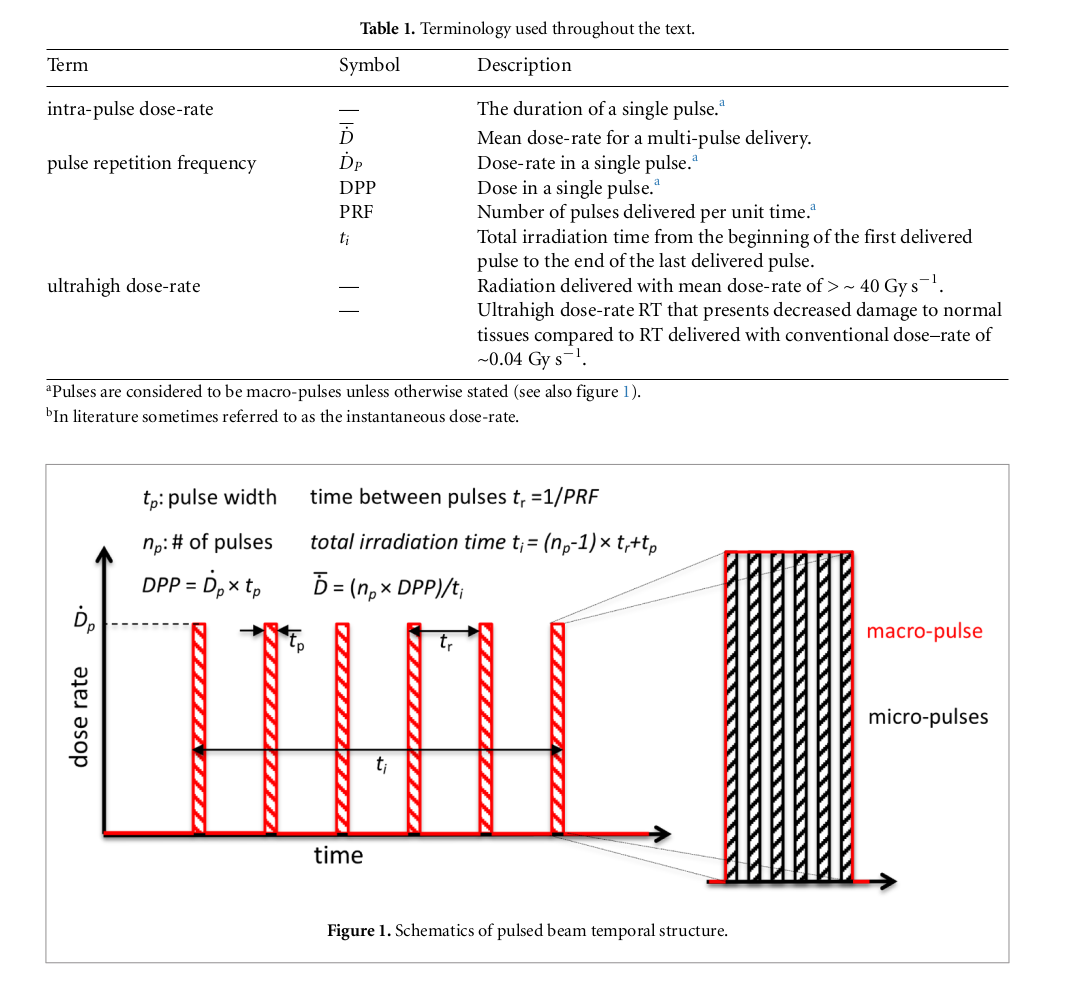
\includegraphics[width=.98\linewidth]{figures/test_beam/dose_param.png}
      \caption{}
      \label{fig:}
   \end{figure}

\section{Apparatus description}


\section{Measurements}
   Numero di hit in funzione del DDP. Spettri con e senza collimatori. 






